\documentclass[12pt,a4paper]{memoir}
% \documentclass[titlepage,12pt,a4paper]{book}

% substituir linha seguinte por 
% \usepackage[english]{babel} 
% se o relatório for escrito na língua inglesa.
\usepackage[portuguese]{babel}

% \usepackage[utf8]{inputenc}
\usepackage[T1]{fontenc}

\usepackage{makeidx}
\usepackage{xspace}
\usepackage{graphicx,color,times}
\usepackage{fancyhdr}
% \usepackage{pxfonts}
% \usepackage{times}
% \usepackage{mathptm}
% \usepackage{amssymb}
% \usepackage{amsfonts}

\usepackage{amsmath}
\usepackage{latexsym}
\usepackage[printonlyused]{acronym}
\usepackage{float}
\usepackage{listings}
\usepackage{tocbibind}
\usepackage{natbib}
\usepackage{hyperref}

% \usepackage{glossaries}
% \makeglossaries

% \renewcommand{\ttdefault}{phv}

\pagestyle{fancy}
\renewcommand{\chaptermark}[1]{\markboth{#1}{}}
\renewcommand{\sectionmark}[1]{\markright{\thesection\ #1}}
\fancyhf{} \fancyhead[LE,RO]{\bfseries\thepage}
\fancyhead[LO]{\bfseries\rightmark}
\fancyhead[RE]{\bfseries\leftmark}
\renewcommand{\headrulewidth}{0.5pt}
\renewcommand{\footrulewidth}{0pt}
\setlength{\headheight}{15.6pt}
\setlength{\marginparsep}{0cm}
\setlength{\marginparwidth}{0cm}
\setlength{\marginparpush}{0cm}
\addtolength{\hoffset}{-1.0cm}
\addtolength{\oddsidemargin}{\evensidemargin}
\addtolength{\oddsidemargin}{0.5cm}
\addtolength{\evensidemargin}{-0.5cm}


\usepackage{fix-cm}
\usepackage{fourier}
\usepackage[scaled=.92]{helvet}
\definecolor{ChapGrey}{rgb}{0.6,0.6,0.6}
\newcommand{\LargeFont}{
  \usefont{\encodingdefault}{\rmdefault}{b}{n}
  \fontsize{60}{80}\selectfont\color{ChapGrey}
  }
\makeatletter
\makechapterstyle{GreyNum}{
  \renewcommand{\chapnamefont}{\large\sffamily\bfseries\itshape}
  \renewcommand{\chapnumfont}{\LargeFont}
  \renewcommand{\chaptitlefont}{\Huge\sffamily\bfseries\itshape}
  \setlength{\beforechapskip}{0pt}
  \setlength{\midchapskip}{40pt}
  \setlength{\afterchapskip}{60pt}
  \renewcommand\chapterheadstart{\vspace*{\beforechapskip}}
  \renewcommand\printchaptername{
  \begin{tabular}{@{}c@{}}
    \chapnamefont \@chapapp\\}
    \renewcommand\chapternamenum{\noalign{\vskip 2ex}}
    \renewcommand\printchapternum{\chapnumfont\thechapter\par}
    \renewcommand\afterchapternum{
  \end{tabular}
  \par\nobreak\vskip\midchapskip}
  \renewcommand\printchapternonum{}
  \renewcommand\printchaptertitle[1]{
  {\chaptitlefont{##1}\par}}
  \renewcommand\afterchaptertitle{\par\nobreak\vskip \afterchapskip}
}
\makeatother
\chapterstyle{GreyNum}

\setcounter{tocdepth}{3}
\setsecnumdepth{subsubsection}

\renewcommand{\ttdefault}{lmtt}


% NEW COLORS
\definecolor{dark}{gray}{0.25}
\definecolor{lgray}{gray}{0.9}
\definecolor{dkblue}{rgb}{0,0.13,0.4}
\definecolor{dkgreen}{rgb}{0,0.6,0}
\definecolor{gray}{rgb}{0.5,0.5,0.5}
\definecolor{mauve}{rgb}{0.58,0,0.82}

\lstset{ %
  language=C,                    basicstyle=\footnotesize,
  numbers=none,                  numberstyle=\tiny\color{gray}, 
  stepnumber=1,                  numbersep=5pt,
  backgroundcolor=\color{white}, showspaces=false,
  showstringspaces=false,        showtabs=false,
  frame=single,                  rulecolor=\color{black},
  tabsize=2,                     captionpos=b,
  breaklines=true,               breakatwhitespace=false,
  title=\lstname,                keywordstyle=\color{blue},
  commentstyle=\color{dkgreen},  stringstyle=\color{mauve},
  escapeinside={\%*}{*)},        morekeywords={*},
  belowskip=0cm
}

\renewcommand{\lstlistingname}{Excerto de Código}
\renewcommand{\lstlistlistingname}{Lista de Excertos de Código}

\renewcommand{\today}{\day \ifcase \month \or Janeiro\or Fevereiro\or Março\or %
Abril\or Maio\or Junho\or Julho\or Agosto\or Setembro\or Outubro\or Novembro\or %
Dezembro\fi de \number \year} 



\begin{document}

\thispagestyle{empty}
\setcounter{page}{-1}

\begin{center}
\begin{Huge}
\textbf{Universidade da Beira Interior}
\end{Huge}
\end{center}

\begin{center}
\begin{Huge}
Departamento de Informática
\end{Huge}
\end{center}

\vspace{0,07cm}
\begin{figure}[!htb]
\centering

\includegraphics[width=191pt]{ubi-fe-di.png}
\end{figure}

\vspace{0.5cm}
\begin{center}
\begin{Large}
\textbf{\theteam: \appname}
\end{Large}
\end{center}

\vspace{0.5cm}
\begin{center}
\begin{normalsize}
\begin{large}
Elaborado por:
\end{large}
\end{normalsize}
\end{center}

\vspace{0.2cm}
\begin{center}
\begin{large}
\begin{tabular}{>{\bfseries}r @{~~---~~} >{\bfseries}l}
	38950 & Diogo José Real Lavareda    \\
	39392 & Joana Elias Almeida         \\
	41266 & Diogo Castanheira Simões    \\
	41358 & Beatriz Tavares da Costa    \\
	41381 & Igor Cordeiro Bordalo Nunes
\end{tabular}
\end{large}
\end{center}

\vspace{0,5cm}
\begin{center}
\begin{normalsize}
\begin{large}
Orientador:
\end{large}
\end{normalsize}
\end{center}

\vspace{0.2cm}
\begin{center}
\begin{large}
\textbf{Professor Doutor Pedro Ricardo Morais Inácio}
\end{large}
\end{center}

\vspace{0.5cm}
\begin{center}
\begin{normalsize}
%\today
22 de maio de 2021
\end{normalsize}
\end{center}

\clearpage{\thispagestyle{empty}\cleardoublepage}

\frontmatter

\chapter*{Resumo}
\label{chap:ack}



\clearpage{\thispagestyle{empty}\cleardoublepage}


\tableofcontents

\clearpage{\thispagestyle{empty}\cleardoublepage}

\listoffigures

% #   ATENÇÃO
% Se não existirem tabelas, comentar as duas linhas seguintes
\clearpage{\thispagestyle{empty}\cleardoublepage}
\listoftables

% #   ATENÇÃO
% Se existirem trechos de código, descomentar as seguintes linhas
% \clearpage{\thispagestyle{empty}\cleardoublepage}
% \lstlistoflistings

\clearpage{\thispagestyle{empty}\cleardoublepage}
\chapter*{Acrónimos}
\label{ch::acro}

\begin{acronym}[CFIUTE]
	\acro{API}{\textit{Application Programming Interface}}
	\acro{APK}{\textit{Android Application Package}}
	\acro{ARGB}{\textit{Alpha-Red-Green-Blue}}
	\acro{CFIUTE}{Centro de Formação Interação UBI Tecido Empresarial}
	\acro{FQDN}{\emph{Fully Qualified Domain Name}}
	\acro{eduroam}{\emph{Education Roaming}}
	\acro{HTML}{\textit{Hypertext Markup Language}}
	\acro{JDK}{\textit{Java Development Kit}}
	\acro{MVC}{\textit{Model-View-Controller}}
	\acro{RSA}{\emph{Rivest-Shamir-Adleman}}
	\acro{SMTP}{\textit{Simple Mail Transfer Protocol}}
	\acro{SSL}{\emph{Secure Sockets Layer}}
	\acro{SWOT}{\textit{Strength, Weakness, Opportunity, and Threat Analysis}}
	\acro{TaC}{\textit{Together Against Cybercrime}}
	\acro{TI}{Tecnologias de Informação}
	\acro{TUI}{\emph{Text-based User Interface}}
	\acro{UC}{Unidade Curricular}
	\acro{UI}{\textit{User Interface}}
	\acro{URI}{\textit{Uniform Resource Identifier}}
	\acro{XML}{\textit{Extended Markup Language}}
\end{acronym}

% \clearpage{\pagestyle{empty}\cleardoublepage}
% \chapter*{Glossário}
\makeglossaries

\newglossaryentry{.NET Framework}
{
  name={.NET Framework},
  description={É uma plataforma para desenvolvimento e funcionamento de aplicações desenvolvida pela Microsoft.}
}

\newglossaryentry{ASP.NET}
{
  name={ASP .Net},
  description={É uma plataforma da Microsoft para o desenvolvimento de aplicações Web e é o sucessor da tecnologia ASP.}
}

\newglossaryentry{CS}
{
  name={C\#},
  description={Lê-se \textit{C Sharp} e é uma linguagem de programação orientada a objectos, desenvolvida pela Microsoft, inicialmente para a plataforma .NET. O C\# é inspirado na junção entre as linguagens C++ e Java.}
}


\newglossaryentry{Java}
{
  name={JAVA},
  description={É uma linguagem de programação orientada a objectos, desenvolvida pela Sun Microsystems na década de 90. Hoje pertence à empresa Oracle.}
}


\newglossaryentry{OpenDMTP}
{
  name={OpenDMTP},
  description={\textit{Open Device Monitoring and Tracking Protocol} é um protocolo e uma \textit{framework} abertos que permite a comunicação bidireccional entre servidores e clientes através da internet.}
}


\newglossaryentry{OpenGTS}
{
  name={Open GTS},
  description={É o primeiro projecto \textit{Open Source} \textit{Web-Based} para controlo de frotas por GPS.}
}


\newglossaryentry{VS2010}
{
  name={Visual Studio 2010},
  description={\textit{Microsoft Visual Studio 2010} é um sistema de desenvolvimento desenvolvido pela Microsoft e é dedicado ao Framework .NET, que contem um conjunto de ferramentas de desenvolvimento projectadas para auxiliar os programadores a enfrentarem desafios complexos.}
}


\newglossaryentry{WebS}
{
	name={Web Service},
	description={Web services são aplicações modulares auto-descritas e auto-contidas, que permitem a integração de sistemas e a comunicação entre aplicações de diferentes tipos.}
}


\newglossaryentry{WebBased}
{
	name={Web Based},
	description={Aplicação desenvolvida para a Web.}
}

\newglossaryentry{Roaming}
{
	name={Roaming},
	description={Define a possibilidade de um utilizador de uma determinada rede obter rede/conecção fora da área geográfica onde foi registado.}
}


\newglossaryentry{Smartphone}
{
	name={Smartphone},
	description={Smartphone é um telefone móvel que contem muitas das principais tecnologias de comunicação e serviços que existem nos computadores pessoais, como acesso a e-mails, serviços de mensagens instantâneas, internet, GPS, entre outros.}
}

\newglossaryentry{TCPIP}
{
	name={TCP/IP},
	description={É um conjunto de protocolos de comunicação entre computadores ligados rede. O nome TCP/IP surge da união entre dois protocolos: o TCP (Transmission Control Protocol) e o protocolo IP (Internet Protocol).}
}

\newglossaryentry{Firewall}
{
	name={Firewall},
	description={É o nome criado para definir um dispositivo para uma rede de computadores que tem como objectivo criar uma política de segurança num determinado ponto de controlo da rede.}
}

\newglossaryentry{JavaScript}
{
	name={JavaScript},
	description={É uma linguagem de programação baseada na linguagem de programação ECMAScript. Actualmente é a linguagem de programação mais utilizada em \textit{``Client-Side''} nos \textit{browsers}.}
}

\newglossaryentry{Flash}
{
	name={Flash},
	description={Desenvolvido pela Macromedia, o Flash é um software utilizado para criação de animações interactivas que funcionam incorporadas em \textit{Browsers}, \textit{Desktop}, \textit{Smartphones}, \textit{Tablets}, e Televisores.}
}


\newglossaryentry{StoredProcedure}
{
	name={Stored Procedure },
	description={É o nome dado a um conjunto de comandos numa base de dados de forma a simplificar a sua utilização.}
}

\newglossaryentry{SQLS}
{
	name={SQL Server 2008},
	description={É um sistema de gestão de base de dados relacional criado pela Microsoft.}
}

\newglossaryentry{Firm}
{
	name={Firmware},
	description={É o conjunto de instruções operacionais programadas directamente no \textit{hardware} de um equipamento electrónico.}
}

\newglossaryentry{browser}
{
	name={Browser},
	description={É um programa de computador que possibilita aos utilizadores uma interacção com documentos virtuais da Internet, também conhecidos como páginas Web.}
}



\clearpage{\thispagestyle{empty}\cleardoublepage}

\mainmatter
\acresetall
\chapter{Introdução}
\label{chap:intro}

\section{Descrição da proposta}
\label{sec::intro:descricao}

A criptografia é uma das estratégias mais importantes para garantir segurança de dados. Atualmente enfrentamos uma era de globalização com ataque a sistemas para roubo de informações privilegiadas, com o intuito de proveito próprio ou venda das mesmas a terceiros, entre outros fins.

Sendo uma temática tão importante e atual, pretende-se levar a mesma ao público geral e poder transmitir a ``magia'' dos desafios criptográficos.

A aplicação \appname~tem como objetivos permitir aos utilizadores registados publicar e resolver desafios criptográficos, bem como tornar-se numa ferramenta educativa na área da criptografia.

% O projeto foi proposto pelo Professor Doutor Pedro Ricardo Morais Inácio no âmbito da cadeira Segurança Informática, lecionada pelo mesmo.


\section{Constituição do grupo}
\label{sec::intro:grupo}

O presente projeto foi realizado pela equipa \textit{C-Team}, constituída pelos elementos listados na Tabela \ref{tab::c-team}.

\begin{table}[!h]
	\centering
	\begin{tabular}{c l >{\itshape}l}
		\toprule
		\textbf{N\textordmasculine} & \textbf{Nome} & \normalfont\textbf{Alcunha} \\
		\midrule
		38950 & Diogo José Real Lavareda    & Lavareda \\
		39392 & Joana Elias Almeida         & Joaninha \\
		41266 & Diogo Castanheira Simões    & Ash      \\
		41358 & Beatriz Tavares da Costa    & Bea      \\
		41381 & Igor Cordeiro Bordalo Nunes & Etileno  \\
		\bottomrule
	\end{tabular}
	\caption[Constituição da equipa \textit{C-Team}]{Constituição da equipa \textit{C-Team}.}
	\label{tab::c-team}
\end{table}



\section{Organização do Documento}
\label{sec::intro:organizacao}

De modo a refletir o projeto realizado, este relatório encontra-se estruturado em cinco capítulos, nomeadamente:

\begin{enumerate}
\item No primeiro capítulo --- \textbf{Introdução} --- são apresentados o projeto, os seus objetivos, a equipa desenvolvedora e a respetiva organização do relatório.

\item No segundo capítulo --- \textbf{Engenharia de Software} --- são elaborados os diagramas de casos de uso da aplicação que orientam a respetiva implementação.

\item No terceiro capítulo --- \textbf{Implementação} --- são descritas as escolhas e os detalhes de implementação da aplicação, bem como as tecnologias utilizadas durante o seu desenvolvimento.

\item No quarto capítulo --- \textbf{Reflexão Crítica e Problemas Encontrados} --- são indicados os objetivos alcançados, quais as tarefas realizadas por cada membro do grupo, assim como são expostos os problemas enfrentados e é feita uma reflexão crítica sobre o trabalho.

\item No quinto capítulo --- \textbf{Conclusões e Trabalho Futuro} --- são analisados os conhecimentos adquiridos ao longo do desenvolvimento do projeto e, em contrapartida, o que não se conseguiu alcançar e que poderá ser explorado futuramente.
\end{enumerate}

\clearpage{\thispagestyle{empty}\cleardoublepage}
\chapter{Engenharia de Software}
\label{ch::engsoft}


\section{Introdução}
\label{sec::engsoft:intro}
Um projeto de sucesso envolve uma preparação prévia exímia. A plataforma \emph{CHALLENGE-ACCEPTED} desenvolvida pela \emph{C-Team} não foi exceção. Foram delineados antecipadamente vários pontos fulcrais, nomeadamente:
\begin{itemize}
	\item Ferramentas e tecnologias (Secção \ref{sec::engsoft:tecnologia}): perante uma equipa de 5 pessoas, foi vital determinar quais as tecnologias a utilizar não só para implementar a aplicação mas também para gerir o trabalho paralelo que iria decorrer;
	\item Requisitos funcionais e não-funcionais (Secção \ref{sec::engsoft:requisitos}): a aplicação deve cumprir uma série de requisitos a fim de poder alcançar os objetivos propostos;
	\item Diagramas de casos de uso (Secção \ref{sec::engsoft:casos-uso}): a fim de se perceber as atividades a desenhar e o respetivo código-fonte que as interliga, diferentes casos de uso foram estudados;
	\item Diagrama de atividades (Secção \ref{sec::engsoft:casos-uso}): este diagrama resume o fluxo de funcionamento da aplicação.
\end{itemize}


\section{Ferramentas e tecnologias utilizadas}
\label{sec::engsoft:tecnologia}

As ferramentas utilizadas no âmbito da realização do projeto, sumariadas na Tabela \ref{tab::ferramentas}, visam três componentes essenciais na sua gestão: 1) linguagem de programação, 2) servidor, 3) administração bd, 4) relatório, 5) controlo de versões.


\begin{table}[!htbp]
	\centering
	\begin{tabular}{p{1cm} l l}
		\toprule
		& {\itshape\bfseries Software} & {\bfseries Versão} \\
		\midrule
		\multicolumn{3}{l}{\bfseries Linguagem de Programação} \\
		& \textit{Python} & 3.8.0 \\
	    \midrule
		\multicolumn{3}{l}{\bfseries Servidor} \\
		& \textit{Microsoft Windows Server} & 2019 \\
		& \textit{MariaDB} & 10.4.18 \\
	    \midrule
		\multicolumn{3}{l}{\bfseries Administração BD} \\
	    & \textit{DBeaver} & 21.0.5 \\
        \midrule
		\multicolumn{3}{l}{\bfseries Relatório} \\
		& \textit{Overleaf} & \\
		\midrule
		\multicolumn{3}{l}{\bfseries Controlo de versões} \\
		& \textit{git} & 2.17.1 \\
		& \textit{GitKraken} & 7.6.1  \\
		\midrule
		\bottomrule
	\end{tabular}
	\caption[Ferramentas utilizadas]{Ferramentas e tecnologias utilizadas, organizadas por categoria.}
	\label{tab::ferramentas}
\end{table}



\section{Requisitos}
\label{sec::engsoft:requisitos}

De forma a ir de encontro aos objetivos propostos do projeto (Secção \ref{sec::intro:descricao}), uma série de requisitos funcionais e não-funcionais foi delineada.

\subsection{Requisitos funcionais}
\label{ssec::engsoft:requisitos:funcionais}

A plataforma deve:

\begin{enumerate}
	\item Possuir um ecrã de boas-vindas e instruções de uso do sistema;
	\item Ter um ecrã de registo e \emph{login} de utilizadores;
	\item Ter uma \textit{homepage} com acesso direto às seguintes funcionalidades:
	\begin{enumerate}
		\item resolução de desafios disponíveis,
		\item propor desafios,
		\item pedir ajuda,
		\item \textit{scoreboard} dos utilizadores,
	\end{enumerate}
	\item Permitir responder a desafios;
	\item Permitir submeter dois tipos de desafios, em que um é de decifra de mensagem e outro de descoberta de mensagem.
\end{enumerate}


\subsection{Requisitos não-funcionais}
\label{ssec::engsoft:requisitos:nao-funcionais}

A plataforma deve:

\begin{enumerate}
	\item Permitir apenas uma tentiva a cada 15 segundos para os desafios cifrados;
	\item Usar assinaturas digitais \ac{RSA};
	\item Ter uma interface gráfica minimalista e (\textit{user-friendly});
	\item Ser segura em termos do armazenamento dos dados na base de dados (se possível cifrar os dados guardados duplamente no caso dos desafios).
\end{enumerate}


\section{Casos de Uso}
\label{sec::engsoft:casos-uso}

Para a plataforma \emph{CHALLENGE-ACCEPTED}, foram identificados os seguintes casos de uso:
\begin{enumerate}
	\item Processo de Registo e \emph{Login} (Figura \ref{fig::casos-uso-regis});
	\item \textit{Homepage} (Figura \ref{fig::casos-uso-homepage});
	\item Processo de propor desafio e cifra de mensagem (Figura \ref{fig::casos-uso-propdesafio});
	\item Processo de responder a desafios (Figura \ref{fig::casos-uso-repdesafio});
	\item Processo de propor desafios do tipo valor de hash (Figura \ref{fig::casos-uso-hash});
\end{enumerate}

Os diagramas foram elaborados com recurso ao serviço \textit{Visual Paradigm}.

\begin{figure}[!htbp]
	\centering
	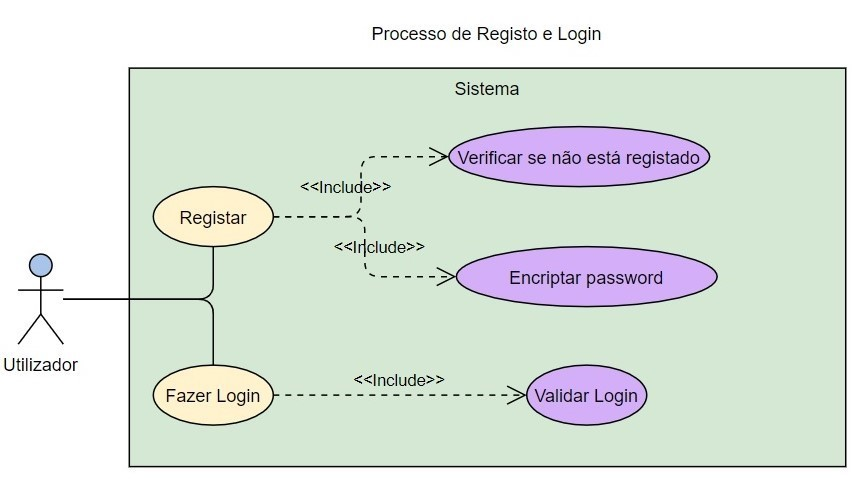
\includegraphics[scale=0.8]{Imagens/Processo_Registo_Login.jpg}	\caption[Diagrama de casos de uso: processo de registo e \emph{Login}]{Diagrama de casos de uso: processo de registo e \emph{Login}}
	\label{fig::casos-uso-regis}
\end{figure}

\begin{figure}[!htbp]
	\centering
	\includegraphics[scale=0.8]{uso-homepage}
	\caption[Diagrama de casos de uso: \emph{homepage}]{Diagrama de casos de uso: \emph{homepage}.}
	\label{fig::casos-uso-homepage}
\end{figure}

\begin{figure}[!htbp]
	\centering
	\includegraphics[scale=0.8]{uso-propdesafio}
	\caption[Diagrama de casos de uso: processo de propor desafio e cifra de mensagem]{Diagrama de casos de uso: processo de propor desafio e cifra de mensagem.}
	\label{fig::casos-uso-propdesafio}
\end{figure}

\begin{figure}[!htbp]
	\centering
	\includegraphics[scale=0.8]{uso-repdesafio}
	\caption[Diagrama de casos de uso: processo de responder a desafios]{Diagrama de casos de uso: processo de responder a desafios.}
	\label{fig::casos-uso-repdesafio}
\end{figure}

\begin{figure}[!htbp]
	\centering
	\includegraphics[scale=0.8]{uso-hash}
	\caption[Diagrama de casos de uso: processo de propor desafios do tipo valor de hash]{Diagrama de casos de uso: processo de propor desafios do tipo valor de hash.}
	\label{fig::casos-uso-hash}
\end{figure}

\section{Diagrama do sistema}
\label{sec::engsoft:diagrama-sistema}

\begin{figure}[!htbp]
	\centering
	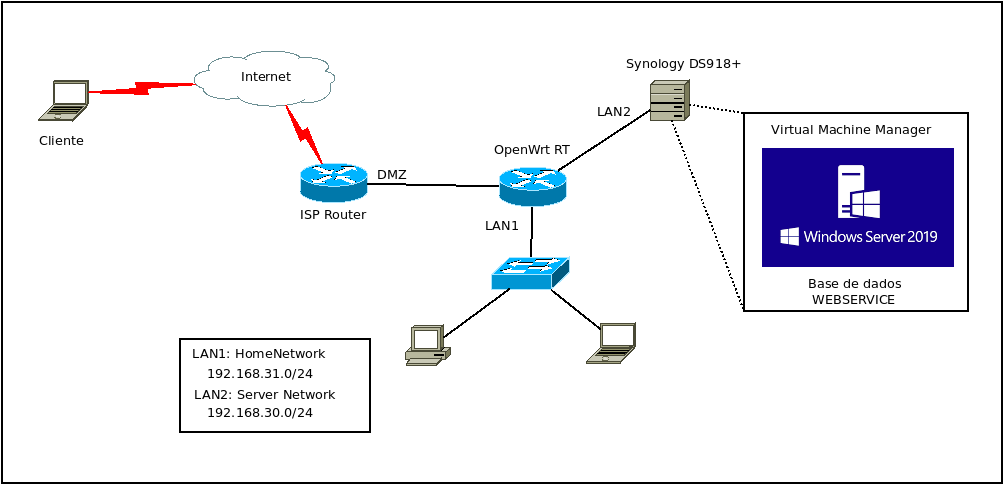
\includegraphics[scale=0.37]{Imagens/DiagramaIdeal.png}	\caption[Diagrama da arquitetura do sistema]{Diagrama da arquitetura do sistema}
	\label{fig::diagrama-sistema}
\end{figure}


\section{Conclusões}
\label{sec::engsoft:conclusao}

Na posse de um plano delineado segundo as práticas comuns da área da Engenharia de \textit{Software}, segue-se a fase de implementação, a qual deve seguir escrupulosamente os requisitos determinados e tem por base os casos de uso estudados. Por fim, o fluxo da aplicação deverá seguir o diagrama de atividades obtido por esta fase de estudo.


\clearpage{\thispagestyle{empty}\cleardoublepage}
\chapter{Tecnologias e Ferramentas Utilizadas}
% OU \chapter{Trabalhos Relacionados}
% OU \chapter{Engenharia de Software}
% OU \chapter{Tecnologias e Ferramentas Utilizadas}
\label{chap:tecno-ferra}

\section{Introdução}
\label{chap3:sec:intro}
Cada capítulo \underline{intermédio} deve começar com uma breve introdução onde é explicado com um pouco mais de detalhe qual é o tema deste capítulo, e como é que se encontra organizado (i.e., o que é que cada secção seguinte discute).

\section{Secções Intermédias}
\label{chap3:sec:...}

A tabela~\ref{tab:exemplo} serve apenas o propósito da exemplificação de como se fazem tabelas em \LaTeX.
%
\begin{table}
\centering
\begin{tabular}{|c|lr|}
\hline
\textbf{campo 1} & \textbf{campo 2} & \textbf{campo 3}\\
\hline
\hline
14 & 15 & 16 \\
\hline	
13 & 13 & 13 \\
\hline
\end{tabular}
\caption{Esta é uma tabela de exemplo.}
\label{tab:exemplo}
\end{table}

\section{Conclusões}
\label{chap3:sec:concs}
Cada capítulo \underline{intermédio} deve referir o que demais importante se conclui desta parte do trabalho, de modo a fornecer a motivação para o capítulo ou passos seguintes.
\clearpage{\thispagestyle{empty}\cleardoublepage}
\chapter{Reflexão Crítica e Problemas Encontrados}
\label{chap:reflexao}

\section{Introdução}
\label{chap4:sec:intro}

Não obstante o bom planeamento feito a priori na fase de engenharia de \emph{software} (descrito no Capítulo \ref{ch::engsoft}), o projeto \emph{Challenge-Accepted}, tal como qualquer outro na área das \ac{TI}, enfrentou alguns contratempos e, com o tempo ao dispor, não se revelou possível almejar todas as ambições inicialmente imaginadas. É preciso, pois, refletir sobre o desenvolvimento deste projeto. 
    
    Neste Capítulo são, portanto, explorados os seguintes tópicos:
\begin{itemize}
\item Objetivos propostos vs. alcançados (Secção \ref{chap4:sec:opvsoa}): compara os objetivos
inicialmente propostos com aqueles que foram concluídos no projeto final;
\item Divisão de trabalho pelos elementos do grupo (Secção \ref{chap4:sec:divisao}): lista as tarefas
realizadas por cada elemento da equipa;
\item Problemas encontrados (Secção \ref{chap4:sec:problemas}): na sequência da Secção \ref{chap4:sec:opvsoa}, explora
os problemas encontrados durante a implementação da aplicação;
\item Reflexão crítica (Secção \ref{chap4:sec:reflexao}): é feita uma \ac{SWOT} em retrospetiva pela equipa acerca do projeto.
\end{itemize}

\section{Objetivos Propostos vs. Alcançados}
\label{chap4:sec:opvsoa}

\begin{table}[!htbp]
	\centering
	\begin{tabular}{p{.65\textwidth} >{\centering\let\newline\\\arraybackslash\hspace{0pt}}m{.25\textwidth}}
		\toprule
		{\bfseries Objetivo proposto} & {\bfseries Alcançado?} \\
		\midrule
		Registo de utilizadores com representação segura da palavra-passe na base de dados & $\bullet$ \\
		Submissão de desafios do tipo cifra de mensagens, codificando-a em \textit{BASE64} & $\bullet$ \\	
		Cálculo de código de autenticação de mensagens que permite verificar se uma mensagem foi bem decifrada ou não & $\bullet$ \\
		Submissão de desafios do tipo valor de \textit{hash}, codificando-a em \textit{BASE64} & $\bullet$ \\
		Resposta a desafios e verificação do sucesso da tentativa  & $\bullet$ \\
		Desafios com cifras AES-128-ECB, AES-128-CBC e AES-128-CTR & $\bullet$ \\
		Desafios com funções de hash MD5, SHA256 e SHA512          & $\bullet$ \\
		Limite de uma tentativa a cada 15 segundos para os desafios de cifra &  \\
		Verificar se uma mensagem foi bem decifrada através de assinaturas digitais RSA & - \\
		Suporte ao algoritmo El Gamal                                           & \\
		Outro tipo de desafios criptográficos                                   & \\
		\bottomrule
	\end{tabular}
	\caption[Objetivos propostos vs. alcançados]{
		Objetivos propostos e respetiva indicação de sucesso.\\
		\textit{Legenda.} $\bullet$ Alcançado em pleno; $\circ$ Alcançado parcialmente. -- Não alcançado.
	}
	\label{tab::objetivos}
\end{table}



\section{Divisão do Trabalho pelos Elementos do Grupo}
\label{chap4:sec:divisao}

\begin{table}[!htbp]
	\centering
	\begin{tabular}{l c c c c c}
		\toprule
		\textbf{Tarefa}                             & \textbf{DL} & \textbf{JA} & \textbf{DS} & \textbf{BC} & \textbf{IN} \\
		\midrule
		Gestão do projeto                           &             &             &             &              &            \\
		Engenharia de Software (requisitos)         &             &             &             &              &             \\
		Engenharia de Software (diagramas)          &             &             &             &              &             \\
		Instalação infraestrutura de suporte        &             &             &             &              &            \\
	    Desenvolvimento da base de dados            &             &             &             &              &            \\
		\textit{Framework} da aplicação (cliente-servidor)   &             &             &             &              &            \\
		Implementação dos algoritmos de cifra       &             &             &             &              &            \\
		Documentação do código                      &             &             &             &              &             \\
		Gestão do repositório \textit{git}          &             &             &             &              &              \\
		Relatório                                   &             &             &             &              &             \\
		Apresentação                                &             &             &             &              &              \\
		\bottomrule
	\end{tabular}
	\caption[Distribuição de tarefas]{
		Distribuição de tarefas pelos elementos do grupo.\\
		\textit{Legenda.}~%
		$\bullet$ principal responsável; $\circ$ auxiliou.
		DL: Diogo Lavareda; JA: Joana Almeida; DS: Diogo Simões; BC: Beatriz Costa; IN: Igor Nunes.
	}
	\label{tab::divisao-trabalho}
\end{table}

\section{Problemas Encontrados}
\label{chap4:sec:problemas}

\subsection{Rede \ac{eduroam} e certificado \ac{SSL}}
\label{chap4:subsec:eduroam}

\textbf{(Alterar a escrita apenas as ideias a enunciar)}\\
Ao testarmos a aplicação na rede \ac{eduroam} onde o presente trabalho será defendido, deparamo-nos com o problema desta rede bloquear as comunicações para porto 3300 utilizado no servidor.
Tambem devido ao servidor não ter um \ac{FQDN} para aplicar certificado \ac{SSL}, desta forma para minimizar as alterações a estrutura do servidor optou-se por separar o \emph{WebService} da base de dados para que a aplicação possa ser executada no ambiente de rede da \ac{UBI}.
A solução inicial foi alterada, tendo sido separado o \textit{Web Service} da base de dados para efeito da apresentação do trabalho \ref{fig::diagrama-sistema-new}.

\begin{figure}[!htbp]
	\centering
	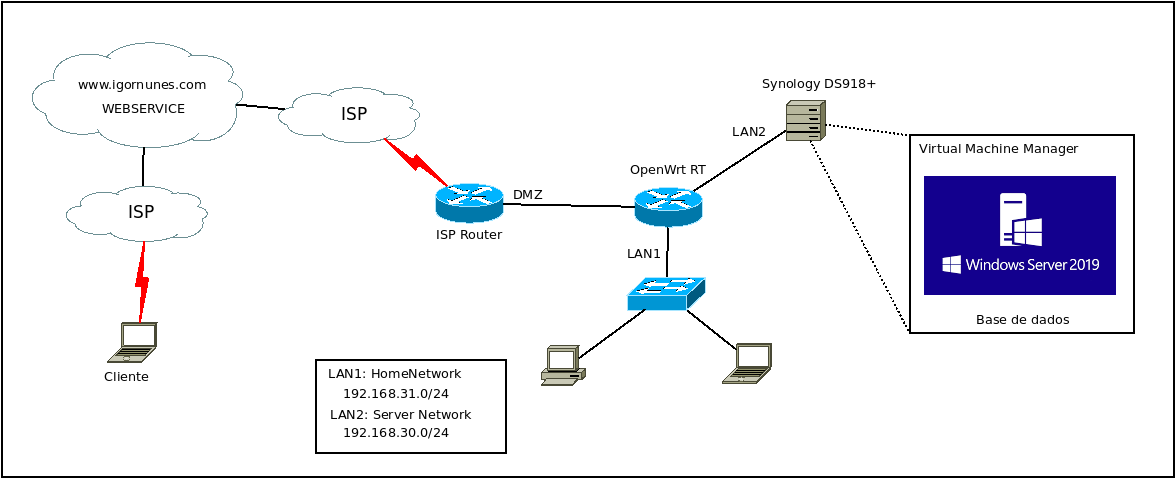
\includegraphics[scale=0.325]{Imagens/DiagramaActual.png}	\caption[Diagrama da arquitetura do sistema atulizado]{Diagrama da arquitetura do sistema atulizado}
	\label{fig::diagrama-sistema-new}
\end{figure}

\section{Reflexão Crítica}
\label{chap4:sec:reflexao}

\subsection{Pontos Fortes}
\label{chap4:subsec:pontosfortes}

\subsection{Pontos Fracos}
\label{chap4:subsec:pontosfracos}

\subsection{Ameaças}
\label{chap4:subsec:ameacas}

\subsection{Oportunidades}
\label{chap4:subsec:oportunidades}

\section{Conclusões}
\label{chap4:sec:concs}
Cada capítulo \underline{intermédio} deve referir o que demais importante se conclui desta parte do trabalho, de modo a fornecer a motivação para o capítulo ou passos seguintes.
\clearpage{\thispagestyle{empty}\cleardoublepage}
\chapter{Conclusões e Trabalho Futuro}
\label{chap:conc-trab-futuro}

\section{Conclusões Principais}
\label{sec:conc-princ}

Esta secção contém a resposta à questão: \\
\emph{Quais foram as conclusões princípais a que o(a) aluno(a) chegou no fim deste trabalho?}

\section{Trabalho Futuro}
\label{sec:trab-futuro}

Esta secção responde a questões como:\\
\emph{O que é que ficou por fazer, e porque?}\\
\emph{O que é que seria interessante fazer, mas não foi feito por não ser exatamente o objetivo deste trabalho?}\\
\emph{Em que outros casos ou situações ou cenários -- que não foram estudados no contexto deste projeto por não ser seu objetivo -- é que o trabalho aqui descrito pode ter aplicações interessantes e porque?}
\clearpage{\thispagestyle{empty}\cleardoublepage}

% SE EXISTIREM APENDICES, DESCOMENTAR O QUE ESTÁ EM BAIXO
% \appendix
% \include{apendice1}
% \clearpage{\pagestyle{empty}\cleardoublepage}
% \include{continuacao}
% \clearpage{\pagestyle{empty}\cleardoublepage}
% \include{apendice2}
% \clearpage{\pagestyle{empty}\cleardoublepage}
% \include{apendice3}
% \clearpage{\pagestyle{empty}\cleardoublepage}

\backmatter

\bibliographystyle{unsrt}
\bibliography{bibliografia}

\end{document}